%background
\chapter{Simulation} 

%\label{ch:bg}

The usual basic requirements to robot simulators are an accurate physics simulation (such as object velocity, inertia, friction, position and orientation, etc.), high quality rendering (for shape, dimensions, colors, and texture of objects), integration with the Robot Operating System (ROS) framework 6 and multiplatform performability. It provides great opportunities for modeling robots and their sensors together with developing robot control algorithms, realizing mobile robot simulation, visualization, locomotion and navigation in a realistic 3D environment. As mentioned in the paper [1], the high graphical fidelity in a robot simulation is important because the sensory input to the robot perceptual algorithms comes from virtual sensors, which are also provided by the simulation. For example, virtual cameras use the simulator rendering engine to obtain their images. If images from a simulated camera have incorrect similarity to real camera ones, then it is not possible to use them for object recognition and localization.

To avoid such a sort of problems, we use the robust and high graphical quality robot simulator - Gazebo, which is an open source robotic simulation package that closely integrated with ROS. Gazebo uses the open source OGRE rendering engine, which produces good graphics fidelity, although it also employs the Open Dynamics Engine (ODE) 7, which is estimated as sufficiently slow physics engine [1].

Integration with ROS gives the access to a large variety of user contributed algorithms. An overview of ROS has been presented in [2].

\section{ROS}

ROS was designed to meet a specific set of challenges encountered when developing large-scale ervice robots as part of the STAIR project [2] at Stanford University1 and the Personal Robots Program [3] at Willow Garage,2 but the resulting architecture is far more general than the service-robot and mobile-manipulation domains.

The philosophical goals of ROS can be summarized as:

\begin{itemize}
\item Peer-to-peer 
\item Tools-based 
\item Multi-lingual 
\item Thin
\item Free and Open-Source
\end{itemize}

\subsection{Nomenclature}

The fundamental concepts of the ROS implementation are nodes, messages, topics, and services.

Nodes are processes that perform computation. ROS is designed to be modular at a fine-grained scale: a system is typically comprised of many nodes. In this context, the term ?node? is interchangable with ?software module.? Our use of the term ?node? arises from visualizations of ROS- based systems at runtime: when many nodes are running, it is convenient to render the peer-to-peer communications as a graph, with processes as graph nodes and the peer-to-peer links as arcs.
Nodes communicate with each other by passing messages. A message is a a strictly typed data structure. Standard primitive types (integer, floating point, boolean, etc.) are supported, as are arrays of primitive types and constants. Messages can be composed of other messages, and arrays of other messages, nested arbitrarily deep.

A node sends a message by publishing it to a given topic, which is simply a string such as ?odometry? or ?map.? A node that is interested in a certain kind of data will subscribe to the appropriate topic. There may be multiple concurrent publishers and subscribers for a single topic, and a single node may publish and/or subscribe to multiple topics. In general, publishers and subscribers are not aware of each others? existence.
The simplest communications are along pipelines:

\subsection{Visualization and Monitoring}

While designing and debugging robotics software, it often becomes necessary to observe some state while the system is running. Although printf is a familiar technique for debugging programs on a single machine, this technique can be difficult to extend to large-scale distributed systems, and can become unwieldly for general-purpose monitoring.
Instead, ROS can exploit the dynamic nature of the connectivity graph to ?tap into? any message stream on the system. Furthermore, the decoupling between publishers and subscribers allows for the creation of general-purpose visualizers. Simple programs can be written which subscribe to a particular topic name and plot a particular type of data, such as laser scans or images. However, a more powerful concept is a visualization program which uses a plugin architecture: this is done in the rviz program, which is distributed with ROS. Visualization panels can be dynami- cally instantiated to view a large variety of datatypes, such as images, point clouds, geometric primitives (such as object recognition results), render robot poses and trajectories, etc. Plugins can be easily written to display more types of data.
A native ROS port is provided for Python, a dynamically- typed language supporting introspection. Using Python, a powerful utility called rostopic was written to filter messages using expressions supplied on the command line, resulting in an instantly customizable ?message tap? which can convert any portion of any data stream into a text stream. These text streams can be piped to other UNIX command- line tools such as grep, sed, and awk, to create complex monitoring tools without writing any code.
Similarly, a tool called rxplot provides the functionality of a virtual oscilloscope, plotting any variable in real-time as a time series, again through the use of Python introspection and expression evaluation.

\begin{figure}[h]
\centering
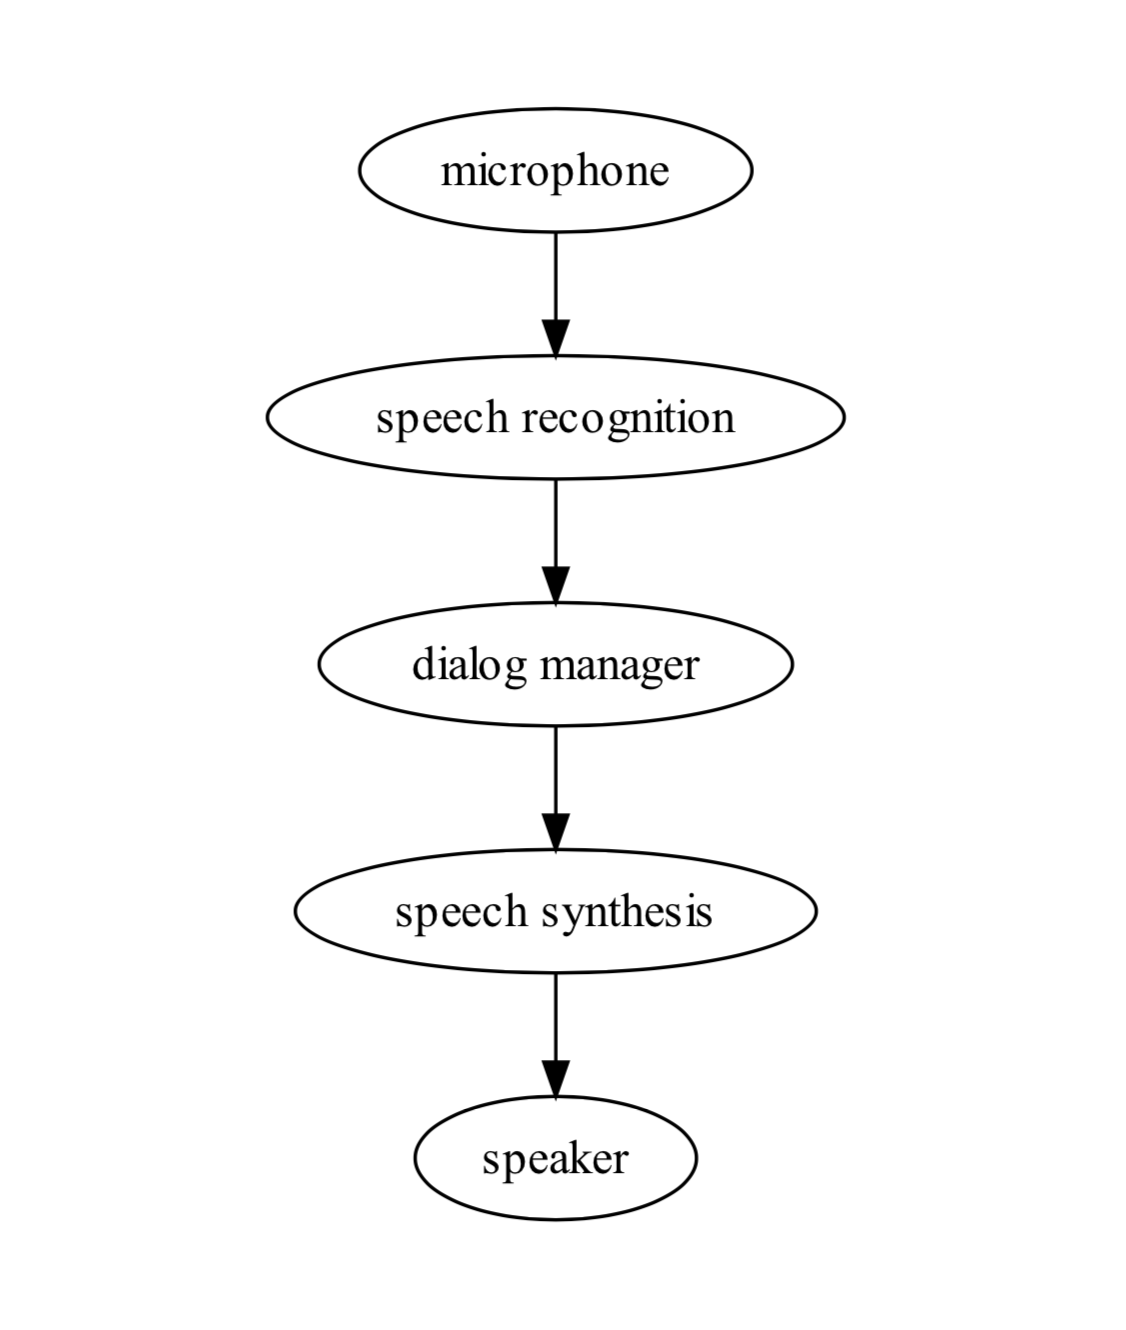
\includegraphics[width=0.5\textwidth]{figs/ch2/ros-pipeline}
\caption{Gazebo for robot simulation.}
\end{figure}

However, graphs are usually far more complex, often containing cycles and one-to-many or many-to-many connections.

Although the topic-based publish-subscribe model is a flexible communications paradigm, its ?broadcast? routing scheme is not appropriate for synchronous transactions, which can simplify the design of some nodes. In ROS, we call this a service, defined by a string name and a pair of strictly typed messages: one for the request and one for the response. This is analogous to web services, which are defined by URIs and have request and response documents of well-defined types. Note that, unlike topics, only one node can advertise a service of any particular name: there can only be one service called ?classify image?, for example, just as there can only be one web service at any given URI.


\subsection{Transformations}

Robotic systems often need to track spatial relationships for a variety of reasons: between a mobile robot and some fixed frame of reference for localization, between the various sensor frames and manipulator frames, or to place frames on target objects for control purposes.
To simplify and unify the treatment of spatial frames, a transformation system has been written for ROS, called tf. The tf system constructs a dynamic transformation tree which relates all frames of reference in the system. As information streams in from the various subsystems of the robot (joint encoders, localization algorithms, etc.), the tf system can produce streams of transformations between nodes on the tree by constructing a path between the desired nodes and performing the necessary calculations.
For example, the tf system can be used to easily generate point clouds in a stationary ?map? frame from laser scans received by a tilting laser scanner on a moving robot. As another example, consider a two-armed robot: the tf system can stream the transformation from a wrist camera on one robotic arm to the moving tool tip of the second arm of the robot. These types of computations can be tedious, error- prone, and difficult to debug when coded by hand, but the tf implementation, combined with the dynamic messaging infrastructure of ROS, allows for an automated, systematic approach.

\section{Gazebo}

Gazebo is a 3D dynamic simulator with the ability to accurately and efficiently simulate populations of robots in complex indoor and outdoor environments. While similar to game engines, Gazebo offers physics simulation at a much higher degree of fidelity, a suite of sensors, and interfaces for both users and programs.

\begin{figure}[h]
\centering
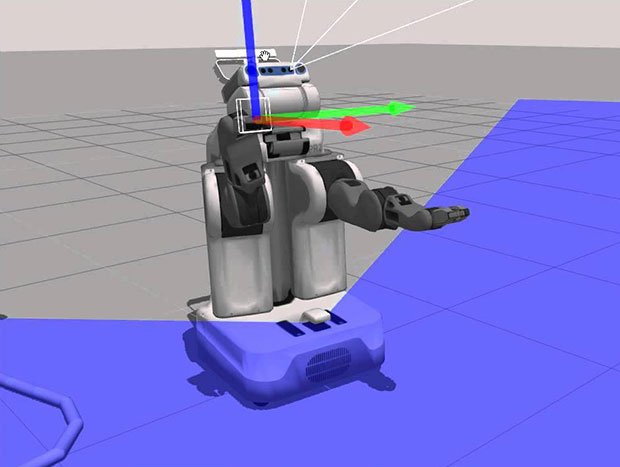
\includegraphics[width=0.5\textwidth]{figs/ch2/osrf.jpeg}
\caption{Gazebo for robot simulation.}
\end{figure}

Typical uses of Gazebo include:

\begin{itemize}

\item testing robotics algorithms,

\item designing robots,

\item performing regression testing with realistic scenarios

\end{itemize}

A few key features of Gazebo include:

\begin{itemize}

\item multiple physics engines,

\item a rich library of robot models and environments,

\item a wide variety of sensors,

\item convenient programmatic and graphical interfaces

\end{itemize}

Gazebo is far from being the only choice for a 3D dynamics simulator. It is however one of the few that attempts to create realistic worlds for the robots rather than just human users. As more advanced sensors are developed and incorporated into Gazebo the line between simulation and reality will continue to blur, but accuracy in terms of robot sensors and actuators will remain an overriding goal.

Robot simulation is an essential tool in every roboticist's toolbox. A well-designed simulator makes it possible to rapidly test algorithms, design robots, perform regression testing, and train AI system using realistic scenarios. Gazebo offers the ability to accurately and efficiently simulate populations of robots in complex indoor and outdoor environments. At your fingertips is a robust physics engine, high-quality graphics, and convenient programmatic and graphical interfaces. Best of all, Gazebo is free with a vibrant community.

\subsection{Architecture}

Gazebo?s architecture has progressed through a couple iterations during which we learned how to best create a simple tool for both developers and end users. We realized from the start that a major feature of Gazebo should be the ability to easily create new robots, actuators, sensors, and arbitrary objects. As a result, Gazebo maintains a simple API for addition of these objects, which we term models, and the necessary hooks for interaction with client programs. A layer below this API resides the third party libraries that handle both the physics simulation and visualization. The particular libraries used were chosen based on their open source status, active user base, and maturity.

This architecture is graphically depicted in Figure 1. The World represents the set of all models and environ- mental factors such as gravity and lighting. Each model is composed of at least one body and any number of joints and sensors. The third party libraries interface with Gazebo at the lowest level. This prevents models from becoming dependent on specific tools that may change in the future. Finally, client commands are received and data returned through a shared memory interface. A model can have many interfaces for functions involving, for example, control of joints and transmission of camera images.

\subsubsection{Physics Engine}

The Open Dynamics Engine [8], created by Russel Smith is a widely used physics engine in the open source com- munity. It is designed to simulate the dynamics and kine- matics associated with articulated rigid bodies. This engine includes many features such as numerous joints, collision detection, mass and rotational functions, and many geome- tries including arbitrary triangle meshes (Figure 6). Gazebo utilizes these features by providing a layer of abstraction situated between ODE and Gazebo models. This layer allows easy creation of both normal and abstract objects such as laser rays and ground planes while maintaining all the functionality provided by ODE. With this internal

abstraction, it is possible to replace the underlying physics engine, should a better alternative become available.

\subsubsection{Visualization}

A well designed simulator usually provides some form of user interface, and Gazebo requires one that is both sophisticated and fast. The heart of Gazebo lies in its ability to simulate dynamics, and this requires significant work on behalf of the user?s computer. A slow and cumbersome user interface would only detract from the simulator?s primary purpose. To account for this, OpenGL and GLUT (OpenGL Utility Toolkit) [9] were chosen as the default visualization tools.
OpenGL is a standard library for the creation of 2D and 3D interactive applications. It is platform indepen- dent, highly scalable, stable, and continually evolving. More importantly, many features in OpenGL have been implemented in graphic card hardware thereby freeing the CPU for other work such as the computationally expensive dynamics engine.
GLUT is a simple window system independent toolkit for OpenGL applications. Scenes rendered using OpenGL are displayed in windows created by GLUT. This toolkit also provides mechanisms for user interaction with Gazebo via standard input devices such as keyboards and mice. GLUT was chosen as the default windowing toolkit be- cause it is lightweight, easy to use, and platform indepen- dent.

\subsubsection{The World}
A complete environment is essentially a collection of models and sensors. The ground and buildings represent stationary models while robots and other objects are dy- namic. Sensors remain separate from the dynamic simula- tion since they only collect data, or emit data if it is an active sensor.
The following is a brief description of each general component involved in the simulator.
1) Models, Bodies, and Joints: A model is any object that maintains a physical representation. This encompasses anything from simple geometry to complex robots. Models are composed of at least one rigid body, zero or more joints and sensors, and interfaces to facilitate the flow of data.
Bodies represent the basic building blocks of a model. Their physical representation take the form of geometric shapes chosen from boxes, spheres, cylinders, planes, and lines. Each body has an assigned mass, friction, bounce factor, and rendering properties such as color, texture, transparency, etc.
Joints provide the mechanism to connect bodies together to form kinematic and dynamic relationships. A variety of joints are available including hinge joints for rotation along one or two axis, slider joints for translation along a single axis, ball and socket joints, and universal joints for rotation about two perpendicular joints. Besides connecting two bodies together, these joints can act like motors. When a force is applied to a joint, the friction between the connected body and other bodies cause motion. However, special care needs to be taken when connecting many joints in a single model as both the model and simulation can easily loose stability if incorrect parameters are chosen.
Interfaces provide the means by which client programs can access and control models. Commands sent over an interface can instruct a model to move joints, change the configuration of associated sensors, or request sensor data. The interfaces do not place restrictions on a model, thereby allowing the model to interpret the commands in anyway it sees fit.
2) Sensors: A robot can?t perform useful tasks without sensors. A sensor in Gazebo is an abstract device lacking a physical representation. It only gains embodiment when incorporated into a model. This feature allows for the reuse of sensors in numerous models thereby reducing code and confusion.
There currently are three sensor implementations including an odometer, ray proximity, and a camera. Odometry is easily accessible through integration of the distance traveled. The ray proximity sensor returns the contact point of the closest object along the ray?s path. This generic sensor has been incorporated into a Sick LMS200 model to simulate a scanning laser range finder, and also into a sonar array for the Pioneer 2. Finally, the camera renders a scene using OpenGL from the perspective of the model it is attached to. Currently the camera sensor is used for both a Sony VID30 camera and the ?god?s eye? view of the world.
3) External Interfaces: Gazebo is generally used in conjunction with Player. The Player device server treats Gazebo as a normal device capable of sending and re-ceiving data. From the users point of view, the models simulated in Gazebo are the same as their real counterparts. A second key advantage to this approach is that one can use abstract drivers inside a simulation. For example, it is possible to use Player?s VFH (Vector Field Histogram) [10] or AMCL (Adaptive Monte-Carlo Localization) [11] interchangeably between real and simulated environments.
The interface to Gazebo is not limited to Player alone. The low-level library provides a mechanism for any third- party robot device server (Player or otherwise) to interface with Gazebo. Going even further, a connection to the the library is not even necessary since Gazebo can be run independently for rapid model and sensor development.
Currently the Gazebo library offers hooks to set wheel velocities, read data from a laser range finder, retrieve images from a camera, and insert simple objects into the environment at runtime. This data is communicated through shared memory for speed and efficiency.

\subsubsection{Construction of Models}

Models are currently created by hand. The process starts with choosing the appropriate bodies and joints necessary to build an accurate model in both appearance and func- tionality. Following Figure 2, we will use the construction of the Pioneer2 AT model as an example. The entire set of bodies for this model encompass four cylinders for the wheels and a rectangular box body.

The next step attaches the bodies together using joints. The end result is a complete physical representation of our model. For the Pioneer2 AT, each wheel has a single axis of rotation. Hinge joints match this requirement perfectly. They are connected to the sides of the rectangular base and the wheels such that the axis of rotation allows for proper wheel spin.

Our Pioneer2 AT model now only lacks an interface for user control. A few functions provided by the Gazebo library resolve this issue, and allow a user to apply velocity changes to the wheels and retrieve odometric data. The Pioneer2 AT model base can also be retro-fitted with any number of devices such as a sonar ring, gripper, and laser range finder.

\section{Vehicle Model}

A well performed vehicle model kit, ADAS Kit Gazebo/ROS Simulator, is adopted here.

\subsection{URDF Models}

\begin{figure}[h]
\centering
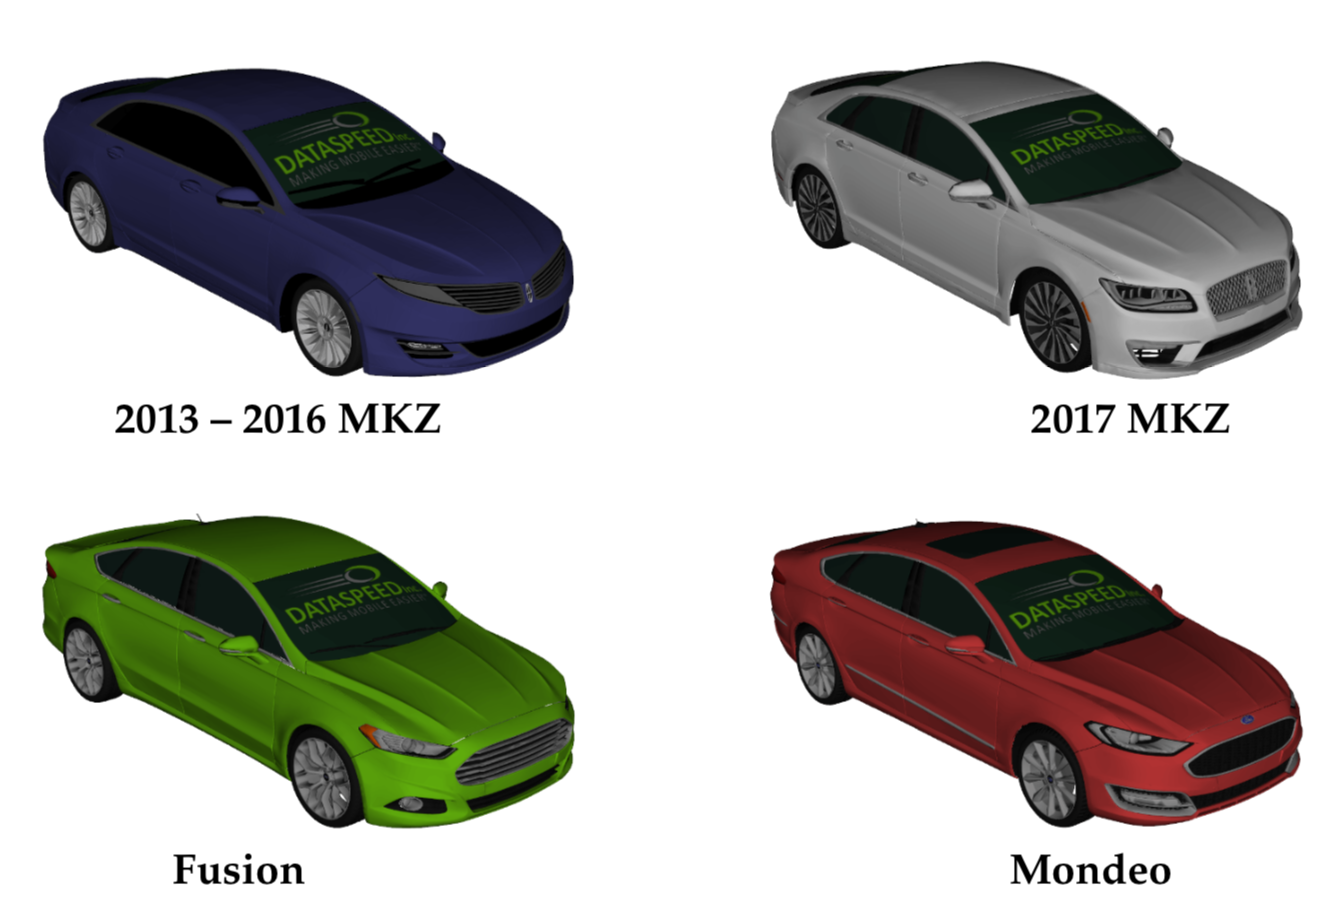
\includegraphics[width=0.5\textwidth]{figs/ch2/mkz-cover}
\caption{A general highway case display.}
\end{figure}

Four URDF models representing the different vehicles supported by the Dataspeed ADAS Kit are included in the simulation. These are shown in Figure 1. The TF trees of the simulation models are all the same, and this common TF tree is shown in Figure 2.

\begin{figure}
\centering
\begin{minipage}{.5\textwidth}
  \centering
  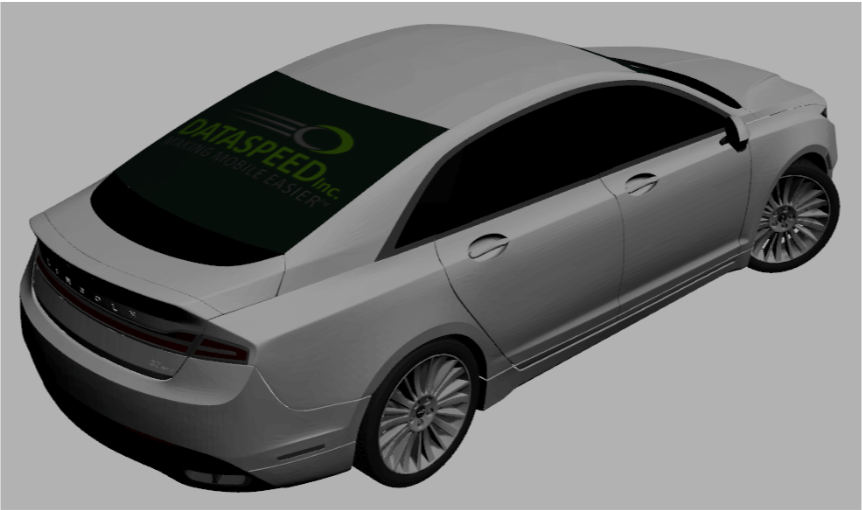
\includegraphics[width=0.9\linewidth]{figs/ch2/mkz-model}
  \label{fig:sub1}
\end{minipage}%
\begin{minipage}{.5\textwidth}
  \centering
  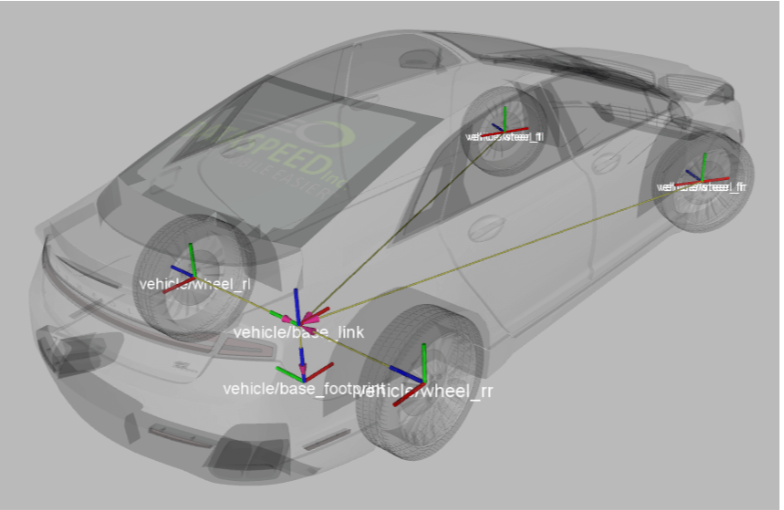
\includegraphics[width=0.82\linewidth]{figs/ch2/mkz-tf-tree}
  \label{fig:sub2}
\end{minipage}
\caption{Simulation model and corresponding TF tree.}
\label{fig:test}
\end{figure}

\subsection{Simulated CAN Message Interface}

The simulator emulates the CAN message interface to the real ADAS Kit. Therefore, there are only two ROS topics used to interact with the simulated vehicle: can bus dbw  can tx to send CAN messages to the vehicle, and can bus dbw  can rx to receive feedback data from the vehicle. These topics and their corresponding message types are listed in Table 2.1.

\begin{table}[h!]
\centering
\begin{tabular}{c c} 
 \hline
 Topic Name & Msg Type \\ [0.5ex] 
 \hline
 $~<name>/can_bus_dbw/can_rx$ & $can_msgs/Frame$  \\ 
 \hline
 $~<name>/can_bus_dbw/can_tx$ & $can_msgs/Frame$ \\ [1ex] 
 \hline \\
\end{tabular}
\caption{CAN message topics to interact with simulated ADAS Kit.}
\label{table:1}
\end{table}

The simulator only implements a subset of the complete Dataspeed CAN message specification. The supported command messages are listed in Table 2.2, and the supported report messages are listed in Table 3. See the ADAS Kit datasheets for complete CAN message information.

\begin{table}[h!]
\centering
\begin{tabular}{c c} 
 \hline
 Command Msg & CAN ID \\ [0.5ex] 
 \hline
 Brake & 0x060 \\ 
 \hline
 Throttle &0x062 \\
  \hline
 Steering & 0x064 \\
 \hline
 Gear & 0x066 \\  [1ex] 
 \hline \\
\end{tabular}
\caption{Command CAN messages supported by the ADAS Kit simulator.}
\label{table:2}
\end{table}

\begin{table}[h!]
\centering
\begin{tabular}{c c c} 
 \hline
Report Msg & CAN ID & Data Rate \\ [0.5ex] 
 \hline
Brake & 0x061 & 50 Hz \\
Throttle & 0x063 &  50 Hz \\
Steering & 0x065 & 50 Hz \\
Gear & 0x067 & 20 Hz \\
Misc & 0x069 & 50 Hz \\
Wheel Speed & 0x06A & 100 Hz \\
Accel & 0x06B & 100 Hz \\
Gyro & 0x06C & 100 Hz \\
GPS1 & 0x6D & 1 Hz \\ 
GPS2 & 0x6E & 1 Hz \\
GPS3 & 0x6F & 1 Hz \\
Brake Info & 0x074 & 50 Hz \\ [1ex]
 \hline \\
\end{tabular}
\caption{Report CAN messages supported by the ADAS Kit simulator.}
\label{table:3}
\end{table}


\subsection{Simulating Multiple Vehicles}

The parameters of the ADAS Kit Gazebo simulation are set using a single YAML file. This section describes the options and formatting of the YAML file.

To simulate multiple vehicles simultaneously, simply add more dictionaries to the array in the YAML file. Below is an example:

\begin{lstlisting}[language=XML]
- vehicle1: 
x: -2.0
y: 0.0
color: red
model: mkz
year: 2017

- vehicle2:
x: 0.0
y: 2.0
color: green
model: fusion
\end{lstlisting}

This would spawn two vehicles: one red 2017 MKZ with model name vehicle1 spawned at (0.0, -2.0, 0.0) and one green 2013 Fusion with model name vehicle2 spawned at (0.0, 2.0, 0.0). Both vehicles would have the default values of the parameters not set in the individual dictionaries.

\section{OpenAI-Gym}

OpenAI Gym aims to combine the best elements of these previous benchmark collections, in a software package that is maximally convenient and accessible. It includes a diverse collection of tasks (called environments) with a common interface, and this collection will grow over time. The environments are versioned in a way that will ensure that results remain meaningful and reproducible as the software is updated.

Alongside the software library, OpenAI Gym has a website (gym.openai.com) where one can find score- boards for all of the environments, showcasing results submitted by users. Users are encouraged to provide links to source code and detailed instructions on how to reproduce their results.

\begin{figure}[h]
\centering
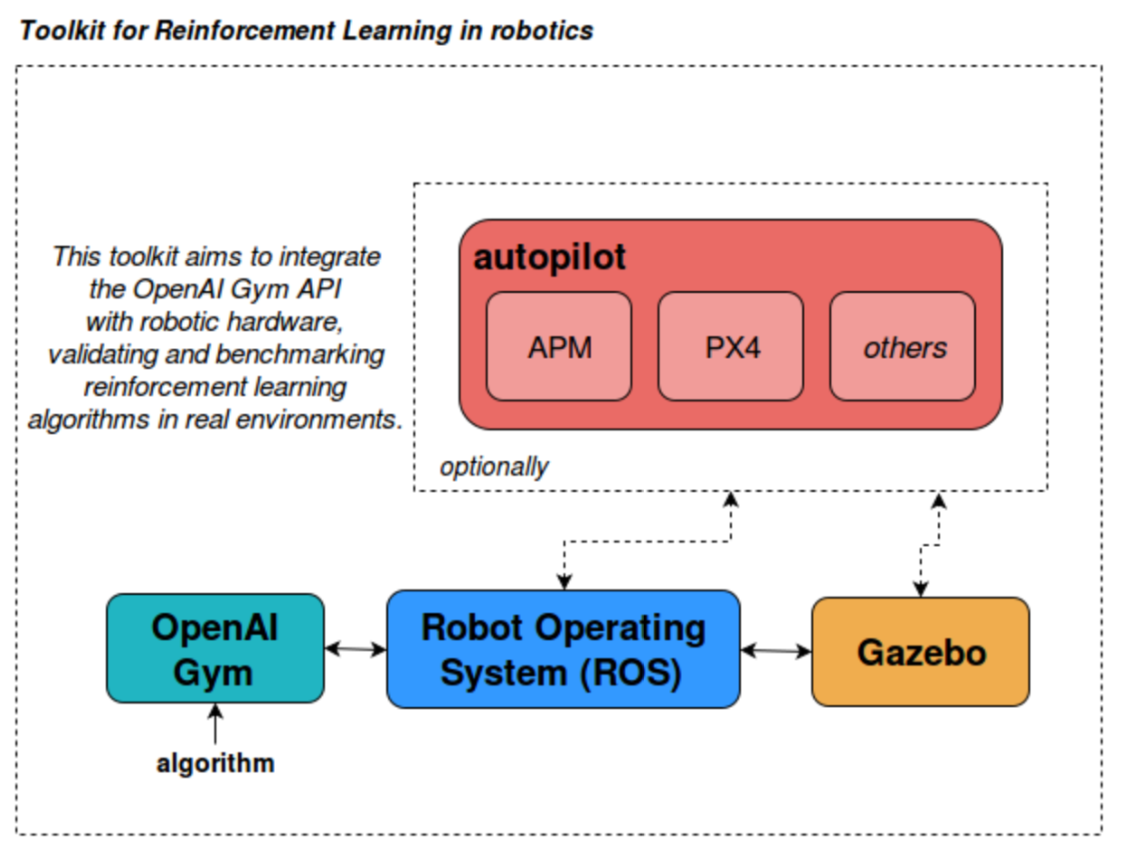
\includegraphics[width=0.5\textwidth]{figs/ch2/toolkit-of-openaigym}
\caption{Simplified software architecture used in OpenAI Gym for robotics..}
\end{figure}

\subsection{Architecture}

The architecture consists of three main software blocks: Ope- nAI Gym, ROS and Gazebo (Figure 1). Environments developed in OpenAI Gym interact with the Robot Operating System, which is the connection between the Gym itself and Gazebo simulator. Gazebo provides a robust physics engine, high-quality graphics, and convenient programmatic and graphical interfaces.

The physics engine needs a robot definition1 in order to simulate it, which is provided by ROS or a gazebo plugin that interacts with an autopilot in some cases (depends on the robot software architecture). The Turtlebot is encapsulated in ROS packages while robots using an autopilot like Erle-Copter and Erle-Rover are defined using the corresponding autopilot. Our policy is that every robot needs to have an interface with ROS, which will maintain an organized architecture.

Figure 1 presents the a simplified diagram of the soft- ware architecture adopted in our work. Our software structure provides similar APIs to the ones presented initially by OpenAI Gym. We added a new collection of environments called gazebo where we store our own gazebo environments with their corresponding assets. The needed installation files are stored inside the gazebo collection folder, which gives the end-user an easier to modify infrastructure.

Installation and setup consits of a ROS catkin workspace containing the ROS packages required for the robots (e.g.: Turtlebot, Erle-Rover and Erle-Copter) and optionally the appropriate autopilot that powers the logic of the robot. In this particular case we used the APM autopilot thereby the source code is also required for simulating Erle-Rover and Erle-Copter. Robots using APM stack need to use a specific plugin in order to communicate with a ROS/Gazebo simulation.

\subsection{Environments and Robots}

We have created a collection of six environments for three robots: Turtlebot, Erle-Rover and Erle-Copter. Following the design decisions of OpenAI Gym, we only provide an abstraction for the environment, not the agent. This means each environment is an independent set of items formed mainly by a robot and a world.

Figure 5 displays an environment created with the Turtlebot robot which has been provided with a LIDAR sensor using and a world called Circuit. If we wanted to test our reinforcement learning algorithm with the Turtlebot but this time using positioning information, we would need to create a completely new environment.

The following are the initial environments and robots pro- vided by our team at Erle Robotics. Potentially, the amount of supported robots/environments will will grow over time.

\subsubsection{Turtlebot.} TurtleBot combines popular off-the-shelf robot components like the iRobot Create, Yujin Robot?s Kobuki, Microsoft?s Kinect and Asus? Xtion Pro into an integrated development platform for ROS applications. For more information, please see turtlebot.com.

\subsubsection{Erle-Rover.} A Linux-based smart car powered by the APM autopilot and with support for the Robot Operating System erlerobotics.com/blog/erle-rover .

\subsubsection{Erle-Copter.} A Linux-based drone powered by the open source APM autopilot and with support for the Robot Oper- ating System erlerobotics.com/blog/erle-copter .

\subsection{Design Decisions}

The design of OpenAI Gym is based on the authors? experience developing and comparing reinforcement learning algorithms, and our experience using previous benchmark collections. Below, we will summarize some of our design decisions.
Environments, not agents. Two core concepts are the agent and the environment. We have chosen to only provide an abstraction for the environment, not for the agent. This choice was to maximize convenience for users and allow them to implement different styles of agent interface. First, one could imagine an ?online learning? style, where the agent takes (observation, reward, done) as an input at each timestep and performs learning updates incrementally. In an alternative ?batch update? style, a agent is called with observation as input, and the reward information is collected separately by the RL algorithm, and later it is used to compute an update. By only specifying the agent interface, we allow users to write their agents with either of these styles.
Emphasize sample complexity, not just final performance. The performance of an RL algorithm on an environment can be measured along two axes: first, the final performance; second, the amount of time it takes to learn?the sample complexity. To be more specific, final performance refers to the average reward per episode, after learning is complete. Learning time can be measured in multiple ways, one simple scheme is to count the number of episodes before a threshold level of average performance is exceeded. This threshold is chosen per-environment in an ad-hoc way, for example, as 90 percent of the maximum performance achievable by a very heavily trained agent.

Both final performance and sample complexity are very interesting, however, arbitrary amounts of computation can be used to boost final performance, making it a comparison of computational resources rather than algorithm quality.
Encourage peer review, not competition. The OpenAI Gym website allows users to compare the performance of their algorithms. One of its inspiration is Kaggle, which hosts a set of machine learning contests with leaderboards. However, the aim of the OpenAI Gym scoreboards is not to create a competition, but rather to stimulate the sharing of code and ideas, and to be a meaningful benchmark for assessing different methods.
RL presents new challenges for benchmarking. In the supervised learning setting, performance is measured by prediction accuracy on a test set, where the correct outputs are hidden from contestants. In RL, it?s less straightforward to measure generalization performance, except by running the users? code on a collection of unseen environments, which would be computationally expensive. Without a hidden test set, one must check that an algorithm did not ?overfit? on the problems it was tested on (for example, through parameter tuning).

We would like to encourage a peer review process for interpreting results submitted by users. Thus, OpenAI Gym asks users to create a Writeup describing their algorithm, parameters used, and linking to code. Writeups should allow other users to reproduce the results. With the source code available, it is possible to make a nuanced judgement about whether the algorithm ?overfit? to the task at hand.
Strict versioning for environments. If an environment changes, results before and after the change would be incomparable. To avoid this problem, we guarantee than any changes to an environment will be accompanied by an increase in version number. For example, the initial version of the CartPole task is named Cartpole-v0, and if its functionality changes, the name will be updated to Cartpole-v1.

\subsubsection{Example Use}


%\bibliographystyle{plainnat}				%Uncomment this if you want a bibliography on each chapter
%\markright{\textit{Bibliography}}
%\renewcommand{\chaptername}{}
%\bibliography{my_references}

%\vfill

